\chapter{Introduction to Computer Control Systems}

\textbf{Resources}
\begin{itemize}
    \item \url{}
\end{itemize}

\newpage

\section{Intro}
\subsection{Control with and without feedback}
\textbf{Control without feedback} is not as common in requires much more
precise models and more sensors in order for it to work. In the case with 
a control for a segway without feedback requires a tone of sensors to measure
every posable input with may change the angle of the handle.

\begin{figure}[!h]
    \centering
    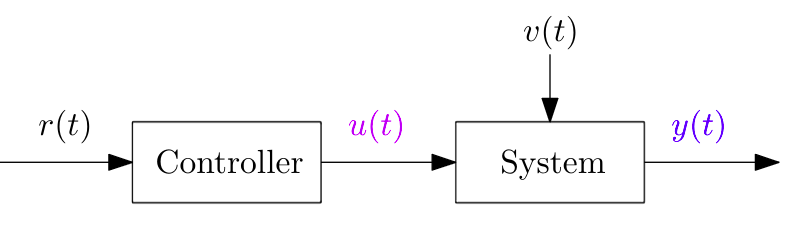
\includegraphics[width=12cm]{\imagesPath/control_without_feedback.png}
    \caption{Control without feedback. From \cite{}}
\end{figure}

\textbf{Control with feedback} is the most common. It is important to have feedback 
since the system rarely accts exactly like the model, for instance if you tell a robot
to drive to a marking and without feedback you have to calculate the voltage needed to
apply to the motors. Meanwhile with feedback you can addjust the stering and voltage 
in reference with the current position.
\begin{figure}[!h]
     \centering
     \begin{subfigure}[b]{0.3\textwidth}
         \centering
         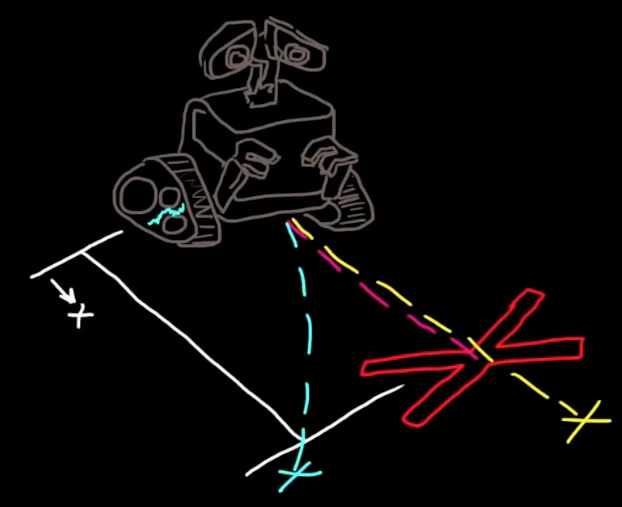
\includegraphics[width=\textwidth]{\imagesPath/feedback_walle}
         \caption{Walle ilustration. From \cite{}}
         \label{fig:y equals x}
     \end{subfigure}
     \hfill
     \begin{subfigure}[b]{0.6\textwidth}
         \centering
         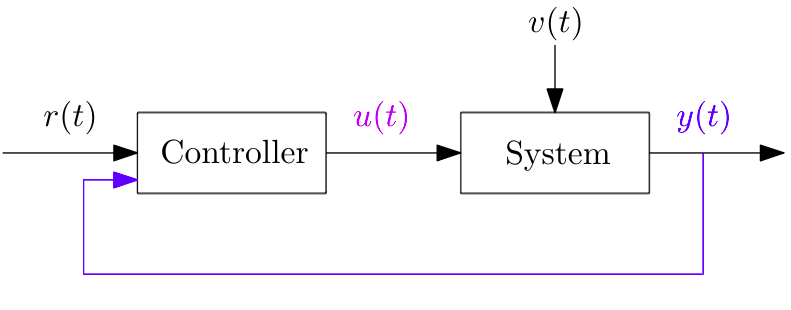
\includegraphics[width=\textwidth]{\imagesPath/control_with_feedback.png}
         \caption{Block diagram. From \cite{}}
         \label{fig:three sin x}
     \end{subfigure}
        \caption{Control with feedback. From \cite{}}
        \label{fig:control_with_feedback}
\end{figure}

The controller part including the reference $r(t)$ is Computer based and the Systems
is generally physical.

\subsection{Typical design requirements}
\begin{enumerate}
    \item \textbf{Stability}: Output $y(t)$ will be \textit{bounded} when reference $r(t)$ is bounded
    \item \textbf{Tracking}: $y(t)$ tracks $r(t)$ \textit{quickly} with minimal \textit{oscillations}
    \item \textbf{Feasibility}: Controller should decide on feasible \textit{input} $u(t)$
    \item \textbf{Robustness}: If a disturbance occurs, output $y(t)$ should quickly \textit{return} to the reference signal $r(t)$.
\end{enumerate}

\subsection{Laplace repetition}
Transforms
Solving ODE 

\subsection{Transfer function of a controller}
\begin{equation*}
    Y(s) = G(s) U(s)
\end{equation*}
see image \ref{fig:control_with_feedback}

The \textbf{Impulse response} is defined as follows
\begin{equation*}
    g(t) = \mathcal{L}^{-1}[G(s)]
\end{equation*}

and
\begin{equation*}
    y(t) = \int_0^t g(\tau) \delta(t-\tau) \equiv g(t)
\end{equation*}

\subsection{Poles and zeros}
The \textbf{zeros} tells us how much the $G(s)$ oscillates and the \textbf{Poles} tells
us how fast it converges. It is \textit{stable} if the poles are negative.

Expressing $G(s)$ via the poles
\begin{equation*}
    G(s)=\frac{B(s)}{A(s)}= \frac{b_1}{s+\sigma_1} + \ldots \frac{B_j(s)}{(s+\sigma_j)^2+\omega_j^2} + \ldots
\end{equation*}

Impulse response then becomes
\begin{equation*}
   g(\tau) = \sum_j b_je^{Re{pole}t} = b_1e^{\sigma_1\tau}+\ldots+b_j\sin(\omega_j\tau+\phi_j)e^{\sigma_j\tau}+\ldots
\end{equation*}

\subsection{Static gain of system}
Assume stable system $Y(s)=G(s)U(s)$ with input $u(t)$ as a step function. $U(s)=\frac{u_0}{s}$

Using the Final value theorem we get the static gain $G(0)$
\begin{equation*}
    y_f  = \lim_{t\to\infty}y(t) = \lim_{s\to 0}Y(s) = lim_{s\to 0}sG(s)\frac{u_0}{s} = G(0)u_0
\end{equation*}
the static gain tells us what value dose the it converges

\begin{exampleblock}{Static gain}
   System
   \begin{equation*}
       G(s)=\frac{2}{s^2 + s + 1}
   \end{equation*}
   where the input to the system is a step response. What is the steady state value dose
   the output have?

   From figure \ref{fig:control_with_feedback} we determine the output as $y(t)=g(t)u(t)$
   \begin{equation*}
        \lim_{t\to\infty}y(t) = \lim_{s\to0} sY(s) = \lim_{s\to0} sG(s)U(s) = \lim_{s\to0} s\frac{2}{s^2 + s + 1}\frac{1}{s} = \frac{2}{1} = 2
   \end{equation*}
\end{exampleblock}

\section{PID control}
\url{https://www.youtube.com/watch?v=UR0hOmjaHp0} \newline
\url{https://www.youtube.com/watch?v=IB1Ir4oCP5k}
\subsection{Feedback control based on error}
\begin{equation*}
    e(t) \triangleq r(t)-y(t)
\end{equation*}

\begin{figure}[!h]
    \centering
    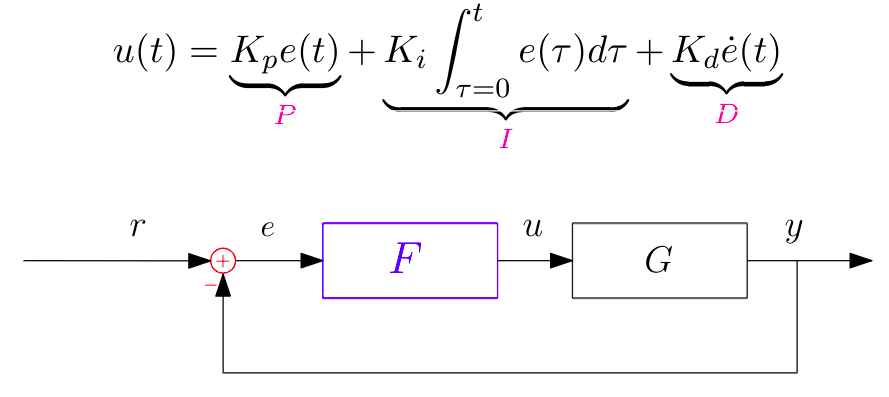
\includegraphics[width=12cm]{\imagesPath/pid-controller.png}
    \caption{PID-controller. From \cite{}}
    \label{fig:pid-controller}
\end{figure}

\begin{itemize}
    \item current error: $\propto e(t)$ (\textbf{P}roportional) \newline 
    The value is the error veted with a constant. How fast the system response.
    \item past error: $\propto \int_{\tau=0}^t e(\tau)d\tau$ (\textbf{I}ntegral) \newline
    The integral under the error from all past values. How fast the steady state error is removed
    \item change in error: $\propto \dot{e}(t)$ (\textbf{D}erivative) \newline
    The rate of change of the error. Faster response and better preforming.
\end{itemize}

using laplace we get:
\begin{align*}
    U(s) &= K_p E(s) + K_i\frac{1}{s}E(s) + K_d s E(s) \\
    &= \Big(K_p + \frac{K_i}{s} + K_d s \Big) E(s) \\
    &= F(s)E(s)
\end{align*}

\begin{itemize}
    \item System from $u$ to $y$: $G(s)$
    \item Closed-loop system from $r$ to $y$: $G_c(s)$
    \item Open-loop system from $e$ to $y$: $G_o(s) = G(s)F(s)$
\end{itemize}

The closed-loop is defined as:
\begin{equation*}
    G_c(s) = \frac{G(s)F(s)}{1+G(s)F(s)}
\end{equation*}

We can define $Y(s)$ as:
\begin{equation*}
    Y(s) = G_c(s) R(s)    
\end{equation*}

The open-loop system is defined as:
\begin{equation*}
    G_o(s) = F(s)G(s)
\end{equation*}

\begin{exampleblock}{Derive close loop}
    Derive $G_c$ TODO
\end{exampleblock}

\textbf{Stationary error}
\begin{align*}
    e_f &= \lim_{t\to\infty}e(t) = \lim_{s\to0}sE(s) \\
    &= \lim_{s\to0}s\frac{1}{1+G_0(s)}\frac{r_0}{s} = \lim_{s\to0} \frac{r_0}{1+G(s)F(s)}
\end{align*}
$e_f$ approaches $0$ if $G(0)F(0)=\infty$. (E.g. when $F(s)$ contains $\frac{1}{s}$, i.e. integration)


\subsection{Classical closed-loop design methods}
%\begin{equation*}
    %Y(s) =\frac{G(s)F(s)}{1 + G(s)F(s)}R(s)
%\end{equation*}
\begin{itemize}
    \item \textbf{Solve roots} of $G_c(s)$ as a function of parameters
    \item \textbf{Routh's algorithm} for Stability check. You only get if the poles are on the left side or not.
    \item \textbf{Root-locus} plot for single parameter
\end{itemize}

\subsubsection{Solve roots}
\begin{exampleblock}{Solve roots}
    The output is expressed as:
    \begin{equation*}
        Y(s) = \frac{4s(s+2)}{s^3+(3+8K_d)^2+(2+8K_p)s+8K_i}V(s)
    \end{equation*}
    what is the poles of the system, if a P-controller is used?

    \begin{align*}
        Y(s) &= \frac{4s(s+2)}{s^3+(3+8K_d)^2+(2+8K_p)s+8K_i}V(s) \\
        &\text{set } K_i = K_d = 0 \\
        &= \frac{4(s+2)}{s^2+3s+2+8K_p}V(s) \\
        &\Rightarrow s^2+3s+2+8K_p = 0  \\ 
        &\Rightarrow s=-1.5 \pm \sqrt{0.25-8K_p} \;\;\; \text{ -using pq-formula}\\
        &\Rightarrow 8K_p > 0.25 \Rightarrow K_p > 0.03125
    \end{align*}
\end{exampleblock}


\subsubsection{Routh's algorithm}
The denominator of the system can be constructed to find the pols, i.e. when the denominator 
is zero.
\begin{equation*}
   a_0s^{n} + b_0s^{n-1} + a_1s^{n-2} + b_1s^{n-3} + \ldots = 0
\end{equation*}
\textbf{Step 1:} construct a table of the coefficient
\begin{center}
    \begin{tabular}{ c c c c c }
     $a_0$ & $a_1$ & $a_2$ & $a_3$ & $\ldots$ \\ 
     $b_0$ & $b_1$ & $b_2$ & $b_3$ & $\ldots$ \\ 
     $c_0$ & $c_1$ & $c_2$ & $\ldots$ & \\ 
    \end{tabular}
\end{center}

\textbf{Step 2:}
\begin{equation*}
    c_k = \frac{b_0a_{k+1} - a_0b{k+1}}{b_0}
\end{equation*}

\begin{exampleblock}{Routh's algorithm}
    The output is expressed as:
    \begin{equation*}
        Y(s) = \frac{4s(s+2)}{s^3+(3+8K_d)^2+(2+8K_p)s+8K_i}V(s)
    \end{equation*}
    is the system stable, if a P-controller is used?

    \begin{equation*}
        G_o(s) = \frac{4s(s+2)}{s^3+(3)^2+(2+8K_p)s}V(s)
    \end{equation*}

    \begin{center}
    \begin{tabular}{ c c c }
     $1$ & $2+8K_p$ & $0$ \\ 
     $1$ & $2+8K_p$ & $0$ \\ 
     $(24K_p+6-8K_i)/3$ & $0$ & $0$ \\
     $(8K_i)$ & $0$ &  \\
    \end{tabular}
    \end{center}

    \begin{align*}
        &\Leftrightarrow 24K_p + 6 - 8K_i > 0 \land K_i > 0 \\
        &\Rightarrow 0 < K_i < \frac{3}{4} + 3K_p
    \end{align*}
\end{exampleblock}


\subsubsection{Rootl-locus}
%\begin{equation*}
%    G_c(s) = \frac{B(s)}{P(s)+KQ(s)}
%\end{equation*}

\begin{exampleblock}{Root-locus algorithm}
    \begin{align*}
        G_0(s) &= \frac{K}{s(s^2 + 2s + 2)} \\
        G_c(s) &= \frac{K}{s(s^2 + 2s + 2) + K.\underbrace{1}_{Q(s)} }
    \end{align*}

    \textbf{Step 1}: Solve the poles $P(s) = s(s^2 + 2s + 2)$
    Starting point (K=0)
    \begin{align*}
        z_{p1} = 0 \\
        z_{p2} = -1+j \\
        z_{p3} = -1-j \\
    \end{align*}

    \textbf{Step 2}: $Q(s) = 1$ 
    Ending points $Q(z_q) = 0$ $\Rightarrow$ no ending points $(K\to\infty)$

    \textbf{Step 3}: Asymptotes
    number of asymptotes $= \;\; \underbrace{\text{number starting}}_{3} \;\; - \;\; \underbrace{\text{number ending}}_{0}$
    the assymptot $\varphi$ 
    \begin{equation*}
        \varphi_A = \frac{2q + 1}{\text{number of asymptotes}}
    \end{equation*}

    \begin{align*}
        \varphi_A(q=0) &= \frac{2\cdot 0 + 1}{3}\cdot\pi = \frac{\pi}{3} \\
        \varphi_A(q=1) &= \frac{2\cdot 1 + 1}{3}\cdot\pi = \pi \\
        \varphi_A(q=2) &= \frac{2\cdot 2 + 1}{3}\cdot\pi = \frac{5\pi}{3} = \frac{-\pi}{3} \\
    \end{align*}

    Intersection of the asymptotes
    \begin{equation*}
        c = \frac{\sum_{p=1} z_p - \sum z_q}{\text{number of asymptotes}} 
        = \frac{0-1+j-1-j}{3}
    \end{equation*}
    see image \ref{fig:root_locus_example}

    \textbf{Step 4}: Intersection with imaginary axis
    \begin{align*}
        &s = 6 + j\omega \\
        &6 = 0 \Rightarrow s = j\omega \\
        &s(s+1)(s+3) + k = 0 \\
        &s^3 + 4s^2 + 3s + k = 0  \\
        \Leftrightarrow &-j\omega^3 - 4\omega^2 + 3j\omega + K = 0 \\
        \Leftrightarrow 
        &\begin{cases}
            K - 4\omega^2 = 0 \\
            w(w^2-3) = 0  
        \end{cases}
        \Rightarrow
        \begin{cases}
            w = 0 \Rightarrow K = 0 \\
            w = \pm\sqrt{3} \Rightarrow K = 12
        \end{cases}
    \end{align*}

    \textbf{Step 5}: Intersection with real axis 
    \begin{align*}
        k &= -s(s+1)(s+3) \\
        \frac{\partial K}{\partial S} &= 0 \Leftrightarrow 3s^2 + 8s + 3 = 0
        &\quad \Rightarrow \textbf{No real solutions}
    \end{align*}
%\begin{align*}
%    Y(s) &= \frac{1}{s+1}U(s) \\
%    U(s) &= (K+\frac{10K}{s})(R(s)-Y(s)) \;\; (K_p=K, K_i=10K) \\ 
%    Y(s) &= \frac{G(s)F(s)}{1+G(s)F(s)}R(s) = \frac{K\frac{s+10}{s(s+1)}}{1+K\frac{s+10}{s(s+1)}}R(s) \\
%    &= \frac{K(s+10)}{s(s+1)+K(s+10)}R(s) \\
%    & \\
%    G_c &= \frac{B(s)}{P(s) + KQ(s)} \\
%    &P(s)+KQ(s) = 0, \;\; 0\leq K \leq \infty \\
%\end{align*}
\end{exampleblock}
\begin{figure}[!h]
    \centering
    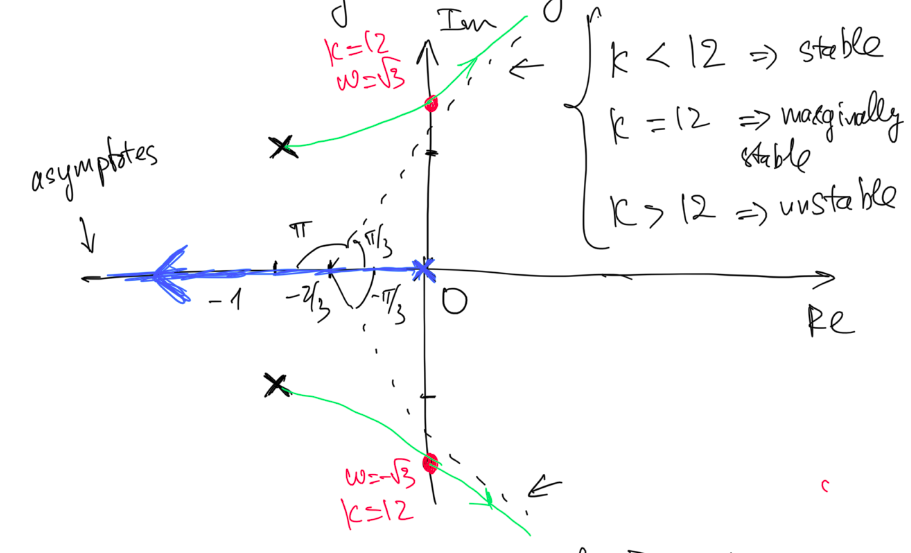
\includegraphics[width=12cm]{\imagesPath/root_locus_example.png}
    \caption{Root locus example}
    \label{fig:root_locus_example}
\end{figure}


% Derive the close gain from a block diagram
% Step response
% PI-control may suppress constant disturbance
% The systems transfer function is that of the closed loop

\section{Good Controller?}
%If the system is already regarded as BIBO stable
\subsection{Method 1: Frequency description of system}
\textbf{Sine in/sine out} principle tels us that the frequency of a signal dose not 
change when applying it to a system (the frequency response dose not change the 
frequency of input signal).

\textbf{System amplitude- and phase plot} tells us how much the system amplifies the 
input signal, mean while the phase plot tells us how much how much it has been moved.

\subsection{Tracking properties of closed-loop system}
Any signal can be represented as a weighted sum of cosine- and sine signals
\begin{equation*}
    r(t) = \frac{1}{2\pi} \int R(i\omega)e^{i\omega t}d\omega
\end{equation*}
recall that $G_c(s)|_{s=i\omega} = G_c(i\omega)$ and that
\begin{equation*}
    Y(i\omega) = G_c(i\omega)R(i\omega) = |G_c(i\omega)|e^{i \arg\{G_c(i\omega)\}}R(i\omega)
\end{equation*}
where ideally the magnitude $|G_c(i\omega)| \approx 1$ and the phase $\arg\{ G_c(i\omega) \} = 0$

Performance metric in time domain:
quickness: rise time $T_r = t_{90\%} - t_{10\%}$
Damping: overshoot $M = (y_{max}- y_f)/y_f$
Accuracy: static control error $e_f = r_0 - y_f$

Performance metric in frequency domain:
quickness: bandwidth $\omega_B$ where $|G_c(i\omega_B)| = |G_c(0)|/\sqrt{2}$
Damping: resonance peak level $M_p = max(|G_c(i\omega)|)$
Accuracy: static gain $G_c(0)$

\subsubsection{Bode plot}
\begin{exampleblock}{Example bode plot}
    \begin{equation*}
        G(s) = \frac{100(s+1)}{s(s^2 + 6s + 100)}
    \end{equation*}

    \textbf{Step 1:} determining the poles and zeros
    \begin{align*}
        \text{Zeros}&: z_1 = -1 \\
        \text{Poles}&: p_0 = 0 \;\; \land \;\; p_1,p_2 = -3\pm i\sqrt{91} = 10
    \end{align*}

    \textbf{Step 2:} sort poles and zeros
    \begin{center}
    \begin{tabular}{ c | c c c c c c } 
      & $|P_0|$ & & $|Z_1|$ & & $P_1$ and $P_2$ & \\ 
     \hline
     $\omega$ & $0$ & & $1$ & & $10$ & \\ 
     slope & & $-1$ & &  $+1$ & & $-2$ \\ 
    \end{tabular}
    \end{center}

    \textbf{Step 3:} draw $\log_{10}(G(i\omega))$ starting at the first pole or zero at the origin
    see figure \ref{fig:example_bode_pot}    
\end{exampleblock}
\begin{figure}[!h]
    \centering
    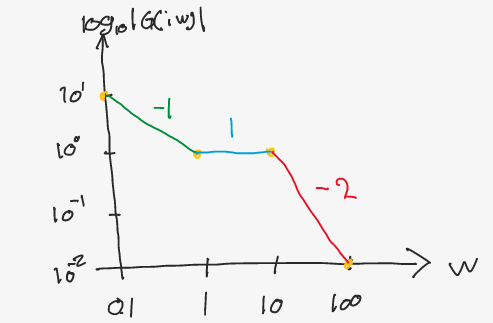
\includegraphics[width=12cm]{\imagesPath/example_bode_plot.png}
    \caption{example bode plot}
    \label{fig:example_bode_pot}
\end{figure}

\subsection{Method 2: Design via open-loop system}
It is easier to design using Open-loop system instead of closed loop with we did in Method 1.

\begin{align*}
    \text{Open-loop: }  &G_o(s) = F(s)G(s) \\
    \text{Closed-loop: }  &G_c(s) = \frac{G_o(s)}{1+G_o(s)} \\
    G_c(s) \text{ stable } \Leftrightarrow 1+&G_o(s) \text{ no roots in right half-plane}
\end{align*}

\subsubsection{Nyquist curve}
\begin{equation*}
    G_o(i\omega) = G(i\omega)F(i\omega), \text{ over } 0 \leq \omega < \infty
\end{equation*}

%\begin{center}
%    \# poles{$G_c(s)$} in right half-plane \newline
%    $=$ \newline
%    \# pole{$G_o(s)$} in right half-plane \newline
%    $+$ Number of positive circles of $\gamma'$ around $-1$
%\end{center}

\begin{figure}[!h]
    \centering
    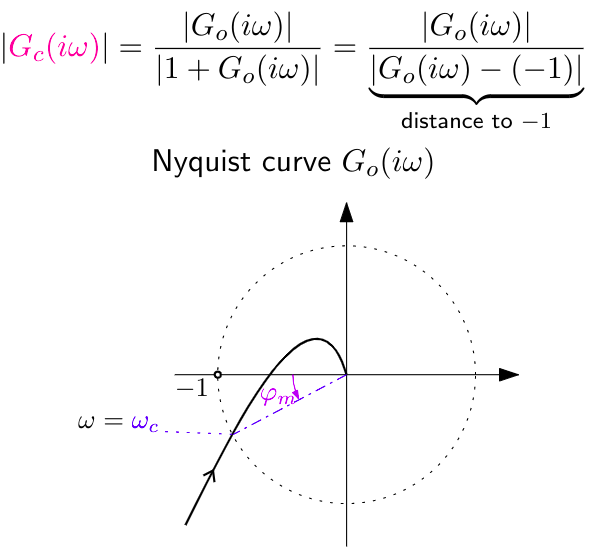
\includegraphics[width=12cm]{\imagesPath/nyquist_curve.png}
    \caption{Nyquist curve. From \cite{}}
    \label{fig:nyquist_curve}
\end{figure}
Note if the \" line is under $-1$ \" then it is stable.
\begin{definitionblock}{\textbf{Crossover frequency} and \textbf{phase margin}}
   Find $\omega = \omega_c$ where $|G_o(i\omega_c)| = 1$ and then define \newline
   $\varphi_m = arg\{ G_o(i\omega_c) + 180^{\circ}$
\end{definitionblock}

The Nyquist curve also tells us quickness and dampining
\begin{itemize}
    \item Crossover frequency $\omega_c \Rightarrow$ bandwidth $\omega_B$ of $G_c$ (quickness)
    \item Phase margin $\varphi_m \Rightarrow$ resonance peak $M_p$ of $G_c$ (damping)
\end{itemize}

Controller $U(s) = F(s)(R(s)-Y(s))$ with three blocks:
\begin{equation*}
    F(s) = K\cdot F_{lead}(s) F_{lag}(s)
\end{equation*}

%Design $G_o$ in the frequency domain:
%\begin{align*}
%    \log_{10} |G_o| &= \log_{10}|G| + log_{10}|F| \\
%    \arg{G_o} &= \arg{G} + \arg{F}
%\end{align*}

Design recipe:
\begin{enumerate}
    \item Initialize with $F_{lead}(s) F_{lag}(s) \equiv 1$ (P-control)
    \item Find a $K$ that yields stable closed-loop system (e.g. via Nyquist criterion)
    \item Adjust $F_{lead}(s)$ and $F_{lag}(s)$ to improve frequency characteristics of $G_o(s)$
\end{enumerate}

Adjust frequency characteristics of open-loop system
\begin{align*}
    \log|G_o(i\omega)| &= \log|G(i\omega)| + \log{K} + \log{|F_{lead}(i\omega)|} + \log{|F_{lag}(i\omega)|} \\
    \arg{G_o(i\omega)} &= \arg{G(i\omega)} + 0 + \arg{|{F_{lead}(i\omega)|} + \arg{F_{lag}(i\omega)}}
\end{align*}

\begin{exampleblock}{Nyquist curve}
    \begin{equation*}
        G_o(s) = \frac{K(s+10)}{s(s^2+3s+50)}
    \end{equation*}
    Denominator: $s(s^2 + 3s + 50)$
    How many roots not LHP

    \textbf{Step 1}
    \begin{equation*}
        s(s^2+3s+50) = 0 \Rightarrow 
        \begin{cases}
            s = 0 \\
            s = -\frac{3}{2} + j\frac{\sqrt{|9|}}{2} \\
            s = -\frac{3}{2} - j\frac{\sqrt{|9|}}{2} \\
        \end{cases}
    \end{equation*}
    see image \ref{fig:nyquist_curve_example_parts}

    \begin{tabular}{ c c c c c c c }
        A  &  $\rightarrow$  &  B  &  $\rightarrow$  &  C  &  $\rightarrow$ & D \\
        $s=j\omega$  &  &  $s=Re^{j\theta}$  &  &  $s=j\omega$  &  &  $s=\epsilon e^{j\theta}$ \\
        $\omega=0^{+}\to\infty$  &  &  $R\to+\infty$  &  &  $\omega:-\infty\to0^{-}$  &  &  $\epsilon\to0$ \\
    \end{tabular}

    \textbf{Step 2}: Investigate each past in open-loop translate function \newline
    Part A: $s=j\omega$ ($\omega:0^{+}\to+\infty$)
    \begin{align*}
        G_A(s=j\omega) &= \frac{K(j\omega + 10)}{j\omega(-w^2+3j\omega+50)}
        = \frac{K(j\omega + 10)}{\omega(-3j\omega+j(50-w^2))} \\
        &= \frac{K(j\omega + 10)(-3\omega - j(50-\omega^2))}{\omega(-9j\omega^2+j(50-w^2)^2)} 
        = \frac{K(20-\omega^2)}{9\omega^ + (50-\omega^2)^2} - j\frac{K(500-7\omega^2)}{\omega(9\omega^2+(50-\omega^2)^2)}
    \end{align*}
    \begin{align*}
        \omega\to0^+: \;\;\; G_A(j0^+) &= \frac{K20}{50^2} - j\infty  \\
        \omega\to+\infty: \;\;\; G_A(j\infty) &= 0 - j0
    \end{align*}

    Intersection of of $G_A(j\omega)$ with real axis 
    \begin{align*}
        &Im[G_A(j\omega)] = 0 & &\Rightarrow w^2 -3 = 0 \\
        & & &\Rightarrow w = \sqrt{3} \\
        &Re[G_A(j\sqrt{3})] = \frac{-K}{18}
    \end{align*}

    Part B: $s = Re^{j\theta}$ $R\to+\infty$
    \begin{align*}
       G_A(s=Re^{j\theta}) &= \frac{K(s+1)}{s^2(s+3)^2} = 0 \\
        &(R\to+\infty)
    \end{align*}

    Part C: and past A are asymmetric around real axis 

    Past D: $s=\epsilon e^{j\theta}$ $\epsilon\to+\infty$
    \begin{align*}
       G_A(s=\epsilon e^{j\theta}) &= \frac{K(s+1)}{s^2(s+3)^2} = \infty \\
        &(\epsilon\to0)
    \end{align*}

    Step 3: see image \ref{fig:nyquist_curve_example_solution}

    Stable $\Leftrightarrow [-1+j0]$ is not enclosed in Nyquist plot
    \begin{align*}
        &\Leftrightarrow -1 < \frac{-K}{18} \\
        &\Rightarrow K < 18
    \end{align*}
\end{exampleblock}

\begin{figure}[!h]
    \centering
    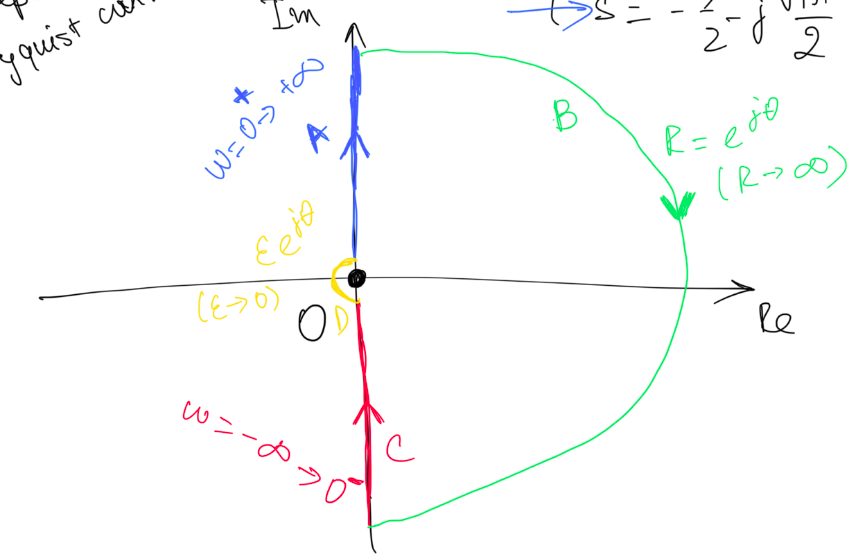
\includegraphics[width=12cm]{\imagesPath/nyquist_curve_example.png}
    \caption{Nyquist curve example}
    \label{fig:nyquist_curve_example_parts}
\end{figure}
\begin{figure}[!h]
    \centering
    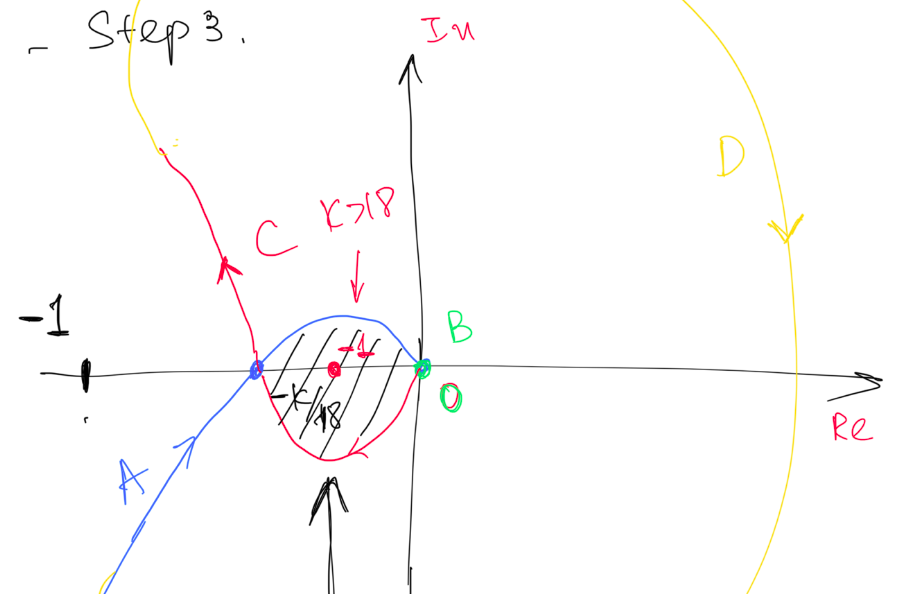
\includegraphics[width=12cm]{\imagesPath/nyqvist_curve_example_solution.png}
    \caption{Nyquist curve example}
    \label{fig:nyquist_curve_example_solution}
\end{figure}

The values for $K$ kan be calculated by (-Negative Intersection * K < 1)


\subsubsection{Minimum phase systems}
\begin{definitionblock}{Definition: Minimum phase system}
   Among all systems $G(s)$ with the same magnitude curve, the system with the 
   least negative phase shift is a \textbf{Minimum phase system} 
\end{definitionblock}
Note: A system is minimum phase $\Leftrightarrow$ it has no poles nor zeros in the 
right half-plane, and contains no time delays.

\subsection{General linear feedback control}
\begin{figure}[!h]
    \centering
    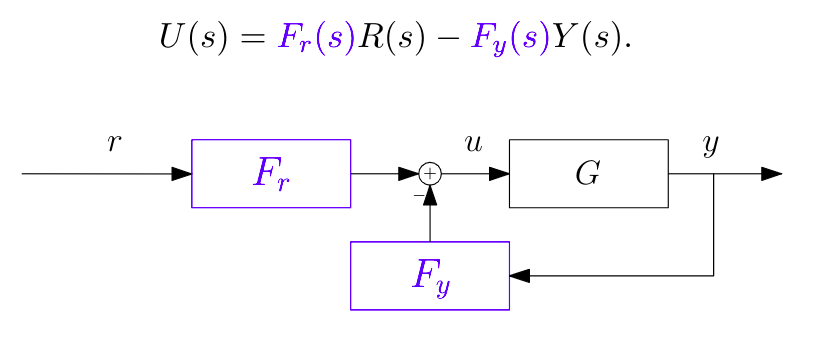
\includegraphics[width=12cm]{\imagesPath/general_linear_feedback_control.png}
    \caption{General linear feedback control. From \cite{}}
    \label{fig:general_linear_feedback_control}
\end{figure}

\begin{equation*}
    Y(s) = \frac{G(s)F_r(s)}{1+G(s)F_y(s)}R(s)
\end{equation*}
Note: $F_y(s) = F_r(s) \equiv F(s) \Rightarrow$ simple linear feedback

\subsubsection{Feedback with measureable disturbances and intermediate signals}
\textbf{Feedback with measureable disturbances}
What if we added more sensors?
\begin{figure}[!h]
    \centering
    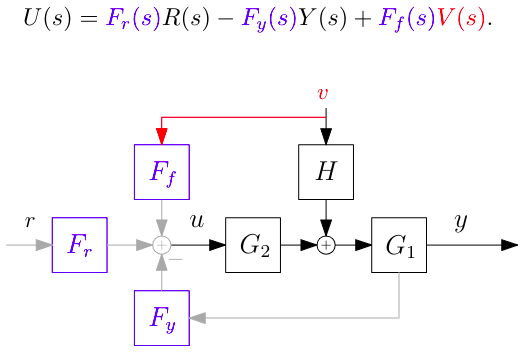
\includegraphics[width=12cm]{\imagesPath/general_feedback_disturbance.png}
    \caption{General feedback with measurable signals including disturbance. From \cite{}}
    \label{fig:general_feedback_disturbance}
\end{figure}

\textbf{Feedback with intermediate signals}
TODO
% F6

\textbf{Combining them}
TODO


\section{Design general linear feedback}
General feedback design methods include:
\begin{enumerate}
    \item Pole placement (using observer)
    \item \sout{Linear quadratic regulation}
    \item \sout{Model predictive control}
\end{enumerate}

\subsection{System states}
\begin{definitionblock}{Definition: system states}
   System states at $t=$ summary of its past from which we can determine the output $y(t)$ 

   Transfer function yields 
   \begin{equation*}
       y(t) = \mathcal{L}^{-1}\{ G(s)U(s) \} = \int_{\tau=0}^{t} g(t)\underbrace{u(t-\tau)}_\text{past input} d\tau
   \end{equation*}

   \begin{align*}
       y(t) &= c_1x_t(t) + c_2x_2(t) + \ldots + c_nx_n(t) + Du(t) \\
       &= Cx(t) + Du(t)
   \end{align*}
   where
   \begin{equation*}
       C = \begin{bmatrix} c_1 & \ldots & c_n \end{bmatrix}
        \text{ and } 
        x(t) \triangleq \begin{bmatrix} x_{1}(t) \\ \vdots \\ x_{n} \end{bmatrix}
   \end{equation*}
\end{definitionblock}

\begin{figure}[!h]
    \centering
    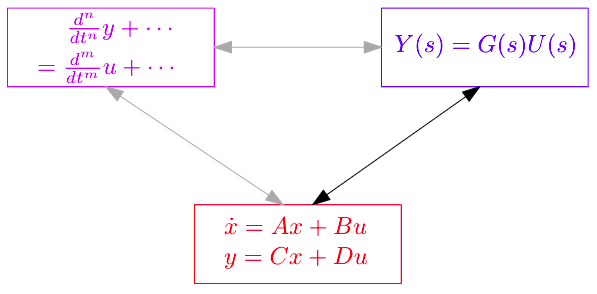
\includegraphics[width=12cm]{\imagesPath/translate_lti_system_models.png}
    \caption{Translate LTI system models. From \cite{}}
\end{figure}

\begin{equation*}
    G(s) = \underbrace{C}_{1\times n}\underbrace{(sI-A)^{-1}}_{n\times n}
    \underbrace{B}_{n\times n} + \underbrace{D}_{1\times 1} = \frac{b(s)}{a(s)}
\end{equation*}

\textbf{Important property}
\begin{itemize}
    \item System matrix A:s eigenvalues $\{\lambda\}$ given by solution to 
    $\det(\lambda I - A) = \lambda^n + a_1\lambda^{n-1} + \ldots a_n = 0$
    \item $a(s) = \det(sI - A)$ is a polynomial of order $n$
    \item $G(s)$:s poles $p_i \subseteq A$:s eigenvalues $\lambda_j$
\end{itemize}

\begin{figure}[!h]
    \centering
    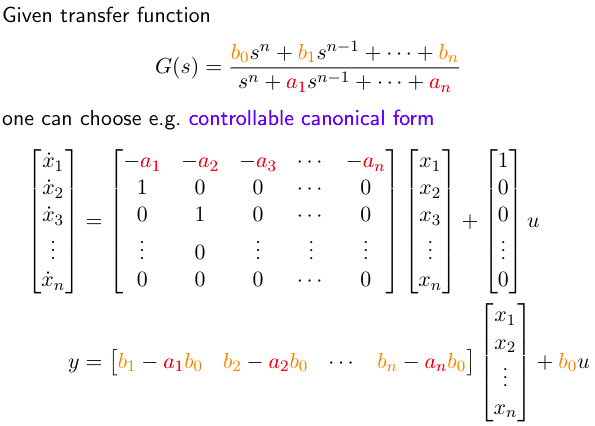
\includegraphics[width=12cm]{\imagesPath/state-space_form_from_transfer_function.png}
    \caption{State-space form $\leftarrow$ transfer function. From \cite{}}
\end{figure}

Solution to state-space equation
\begin{equation*}
    x(t) = e^{At}x_0 + \int_{0}^{t} e^{A\tau} Bu(t-\tau)d\tau
\end{equation*}
matrix exponential $e^{At}$ defined as
\begin{equation*}
    e^{At} = \mathcal{L}^{-1}\left\{ (sI-A)^{-1} \right\}
\end{equation*}

\begin{itemize}
    \item States $x(t)$ at $t$ summarize all past inputs $u(t-\tau)$
    \item State space formulation easily incorporates initial condition
    \item Determine output $y(t) = Cx(t) + Du(t)$
\end{itemize}

Asymptotically stable if 
\begin{equation*}
    u(t) \equiv 0 \Rightarrow \lim_{t\to\infty} x(t) = 0
\end{equation*}

\textbf{stability}
\begin{itemize}
    \item A:s eigenvalues are strictly in left half-plane $\Leftrightarrow$ system is asymptotically stable.
    \item A:s eigenvalues are strictly in left half-plane $\Rightarrow$ system is input-output stable.
\end{itemize}

\begin{exampleblock}{Example: State space}
   TODO  Find transfer function F8 s14
\end{exampleblock}
% example of root locus 
% example of nyqvist 

\section{Nonlinear time-invariant system}
\textbf{Feedback control using states}
\begin{align*}
    \begin{aligned} 
        \dot{x} &= Ax + Bu \\
        y &= Cx 
    \end{aligned}& && \Leftrightarrow \;\; Y(s) = G(s)U(s) \\
\end{align*}
\begin{figure}[!h]
    \centering
    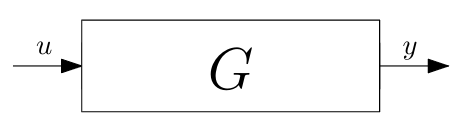
\includegraphics[width=12cm]{\imagesPath/state-feedback_control.png}
    \caption{State-feedback control. From \cite{}}
\end{figure}

\textbf{State space description:}
\begin{align*}
    \begin{aligned}
        \dot{x} &= Ax + Bu \\
        y &= Cx \\
    \end{aligned}&
    && \Leftrightarrow \;\; G(s) = C(sI-A)^{-1}B \\
\end{align*}
\begin{figure}[!h]
    \centering
    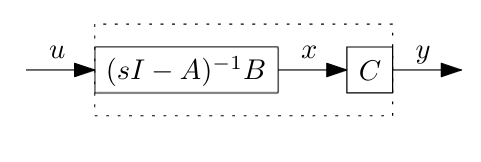
\includegraphics[width=12cm]{\imagesPath/state-feedback_control_2.png}
    \caption{State-feedback control. From \cite{}}
\end{figure}

\begin{equation*}
    u = -Lx + l_0 r
\end{equation*}
\begin{figure}[!h]
    \centering
    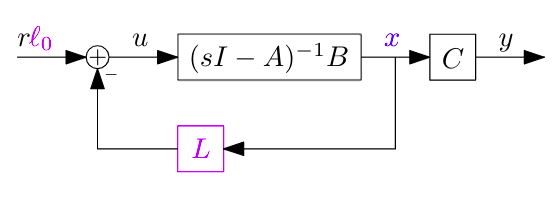
\includegraphics[width=12cm]{\imagesPath/state-feedback_control_3.png}
    \caption{State-feedback control. From \cite{}}
\end{figure}

\textbf{state-space equation:}
\begin{equation*}
    \dot{x} = Ax + B(-Lx+l_0r) = (A-BL)x + Bl_0r
\end{equation*}

The resulting open loop system
\begin{align*}
    \dot{x} &= (A-BL)x + Bl_0r \\
    y &= Cx
\end{align*}

\subsubsection{Controllabel?}
A sought state $x^*$ is \textit{controllable} if we can move the system from $x(0)=0$
to $x(T) = x^*$
\begin{align*}
    x(T) &= e^{At}x_0 + \int_0^T e^{A\tau}Bu(T-\tau)d\tau \\ 
    &= B\gamma_0 + AB\gamma_1 + \ldots + A^{n-1}B\gamma_{n-1}
\end{align*}

\begin{equation*}
    S \triangleq [B \; AB \; \ldots \; A^{n-1}B]
\end{equation*}

All states $x^*$ are controllable $S$:s columns are linearly independent.
$rank(S) = n$ or $\det(S) \neq 0$

\begin{align*}
    y(t) &= Cx(t) \\
    &= Ce^{At}x^* + 0
\end{align*}
\begin{equation*}
    Cx^* = 0, \; CAx^*, \ldots , CA^{n-1}=0
\end{equation*}

\begin{equation*}
    O \triangleq  \begin{bmatrix} C \\ CA \\ \vdots \\ CA^{n-1} \end{bmatrix}
\end{equation*}

\subsubsection{Observable?}
All states $x^*$ are \textit{observable} $\Leftarrow O$:s columns are linearly independent

\begin{exampleblock}{Example: controllable}
   Is the following system controllable?
   \begin{align*}
       x(t) &= \begin{bmatrix} -2 & -1 \\ 1 & 0 \end{bmatrix}x(t) 
       + \begin{bmatrix} 1 \\ 0 \end{bmatrix}u(t) \\ 
       y(t) &= \begin{bmatrix} 1 & 1 \end{bmatrix}x(t)
   \end{align*} 


   \begin{align*}
       \mathcal{O} &= \begin{bmatrix} C \\ CA \\ \vdots \\ CA^{n-1} \end{bmatrix} 
        = [n=2] = \begin{bmatrix} C \\ CA \end{bmatrix} 
        = \underbrace{\begin{bmatrix} C \\ CA \end{bmatrix}}_{2\times2} 
        = \begin{bmatrix} 1 & 1 \\ -1 & -1 \end{bmatrix} \\
        &\Rightarrow \det(\mathcal{O}) 
        =\det\left( \begin{bmatrix} 1 & 1 \\ -1 & -1 \end{bmatrix} \right) 
        = (1)(-1) -(1)(-1) = 0
   \end{align*}
   Therefore the system is not controllable
\end{exampleblock}

\subsection{Minimal realization of state-space form}
State-space form of $G(s)$ is a \textit{minimal realization} if vector $x$ has the 
smallest possible dimension.

A state-space form is \textit{minimal realization} $\Leftrightarrow$ controllable and 
observable $\Leftrightarrow$ $A$:s eigenvalues $= G(s)$:s poles 

\subsection{Method: Design of state-feedback control}
State-space model with controller $u=-Lx+l_0r$ where
\begin{equation*}
    L = \begin{bmatrix} l_1 & l_2 & \ldots & l_n \end{bmatrix}
\end{equation*}

The closed loop system is expressed as
\begin{align*}
    \dot{x} &= (A-BL)x + Bl_0r \\ 
    y &= Cx 
\end{align*}

The closed loop system as a transfer function
\begin{equation*}
    G_c(s) = C(sI-A+BL)^{-1} Bl_0 
\end{equation*}

Calculations of eigenvalues/poles
\begin{equation*}
   \det(sI-A+BL) = 0
\end{equation*}

\begin{equation*}
    l_0 = \frac{1}{C(-A+BL)^{-1}B}
\end{equation*}

State-space form is controllable $\Leftrightarrow L$ can be designed to yield
arbitrarily placed poles (real and complex-conjugated) of the
closed-loop system

\subsection{Estimation via simulation}
Controller
\begin{equation*}
    u = -L\hat{x} + l_0r
\end{equation*}
where $\hat{x}$ is an estimate of the actual state $x$ that is unknown

we estimate via simulating the states
\begin{equation*}
    \dot{\hat{x}} = A\hat{x} + Bu, \;\;\; \hat{x}(0) = \hat{x}_0
\end{equation*}
where $\hat{x}_0$ is an initial guess.

\subsubsection{Estimation vi observer}
Instead of simply guessing what $\hat{x}$ is. 
We use a so called observer

\begin{equation*}
    \dot{\hat{x}} = A\hat{x} + Bu + \underbrace{K(y-C\hat{x})}_{correction}, \;\;\; \hat{x}(0) = \hat{x}_0
\end{equation*}

where $K$ is a matrix

\begin{equation*}
    K = \begin{bmatrix} k_1 \\ k_2 \\ \vdots \\ k_n \end{bmatrix}
\end{equation*}

\begin{figure}[!h]
    \centering
    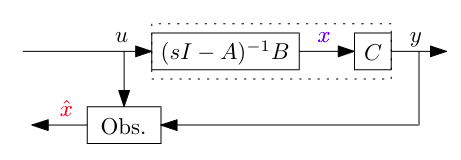
\includegraphics[width=12cm]{\imagesPath/observer_etimating.png}
    \caption{Estimating the states with observer. From \cite{}}
\end{figure}

\subsubsection{Estimation error}
\begin{definitionblock}{Definition: Estimation error}
    \textit{Estimation error:}
    \begin{equation*}
        \tilde{x} \triangleq x-\hat{x}
    \end{equation*}
    Errors of observer described as system 
    \begin{equation*}
        \tilde{x}(t) = e^{(A-KC)t}\tilde{x}(0)
    \end{equation*}
    and therefore $||\tilde{x}(t)||$ decays at a rate given by maximum
    \begin{equation*}
        Re\{\tilde{s}_i\}
    \end{equation*}
    where $\tilde{s}_i$ are observer poles/eigenvalues of $(A-KC)$ 
\end{definitionblock}

State-space form is observable ($\det{\mathcal{O}}\neq0$) $\Rightarrow$ matrix $K$ can
be chosen such that $\tilde{x}$ vanish arbitrarily quick.

$K$ is solved by polynomial $\det(sI-A+KC)=0$ with desired roots in left halfplane

\subsubsection{Controller using estimated states}
\begin{figure}[!h]
    \centering
    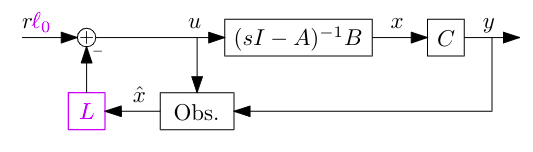
\includegraphics[width=12cm]{\imagesPath/controller_with_observer.png}
    \caption{Estimating the states with observer. From \cite{}}
\end{figure}

\begin{equation*}
    \begin{cases}
        \dot{x} = Ax + Bu \\
        y = Cx \\
    \end{cases}
    \begin{cases}
       u = -L\hat{x} + l_0r \\
       \dot{\hat{x}} = A\hat{x} + Bu + K(y-C\hat{x})
    \end{cases}
\end{equation*}

\begin{equation*}
    L: 
    \begin{cases}
        U(s) = -L\hat{X}(s) + l_0R(s) \\
        s\hat{X}(s) = A\hat{X}(s) + BU(s) + K(Y(s) - C\hat{X}(s))
    \end{cases}
\end{equation*}

\subsubsection{Closed-loop system with estimated states}
Close loop system
\begin{align*}
    \dot{x} &= (A-BL)x + \overbrace{BL\tilde{x}}^{\text{effect of estimation error}} + Bl_0r \\
    y &= Cx
\end{align*}

The closed-loop system with estimation error can be written as 
\begin{align*}
   \begin{bmatrix} \dot{x} \\ \dot{\tilde{x}} \end{bmatrix} &= 
   \underbrace{\begin{bmatrix} A-BL & BL \\ 0 & A-KC \end{bmatrix}}_{\tilde{A}}
   \begin{bmatrix} x \\ \tilde{x} \end{bmatrix} 
   +\underbrace{\begin{bmatrix} B \\ 0 \end{bmatrix}l_0}_{\tilde{B}}r \\
    y &= \underbrace{\begin{bmatrix} C 0 \end{bmatrix}}_{\tilde{C}}
    \begin{bmatrix} x \\ \tilde{x} \end{bmatrix}
\end{align*}

\section{Sensitivity and robustness}
Sensitivity function:
\begin{equation*}
    S(s) \triangleq \frac{1}{1+G_o(s)}
\end{equation*}

Complementary sensitivity function:
\begin{equation*}
    T(s) \triangleq 1-S(s) = \frac{G_o(s)}{1+ G_o(s)}
\end{equation*}

\begin{equation}\label{eq:s_and_t}
    S(s) + T(s) \equiv 1 \;\;\; \forall 1
\end{equation}

\begin{figure}[!h]
    \centering
    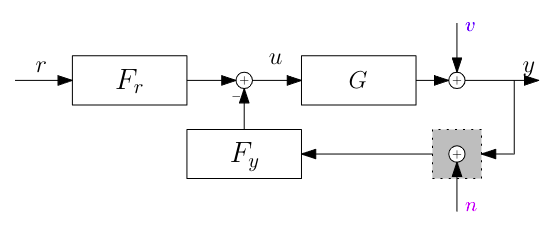
\includegraphics[width=12cm]{\imagesPath/control_system_with_disturbances_and_noise.png}
    \caption{Control system with disturbances and noise. From \cite{}}
\end{figure}

\begin{equation*}
    Y(s) = G_c(s)R(s) + S(s)V(s) + T(s)N(s)
\end{equation*}
where $V(s)$ is the disturbance from external factors on the system. For example a wind 
or other forces. $N(s)$ is the noise witch can be the for example from an inaccurate sensor 
or the sensor not coping with the quick changes.

We can either minimize the disturbance or the noise since $S(s)$ and $T(s)$ are connected
see equation \ref{eq:s_and_t}. Often the noise is high frequency and disturbance is lower
frequency for example if somone is pusing the system the that is a log

Ideally both $|S(i\omega)|$ and $T(i\omega) \gg 1$ 
\begin{equation*}
    |S(i\omega)| + |T(i\omega)| \geq |S(i\omega) + T(i\omega)| \equiv 1
\end{equation*}

In addition we want Nyquist contour
\begin{equation*}
    G_o(i\omega) = F_y(i\omega)G(i\omega) = \frac{T(i\omega)}{S(i\omega)}
\end{equation*}

\subsection{Robustness: model error and stability}
Assume
\begin{enumerate}
    \item Controller $F(s)$ stability the assumed system $G(s)$
    \item $G(s)$ and $G^0(s)$ have same number of poles in right half-plane.
    \item Open-loop: $F(s)G(s)\to0$ and $F(s)G^0(s)\to0$ where $|s|\to\infty$
\end{enumerate}

Robustness criterium 
If assumptions are valid and $T(i\omega)$ fulfills
\begin{equation*}
    |T(i\omega)| < \frac{1}{|\delta G(i\omega)|}, \;\;\; -\infty\leq\omega\leq\infty
\end{equation*}
$\Rightarrow$ the real closed-loop system $G^0_c(s)$ is also stable!


\section{Digital Controllers}
\begin{figure}[!h]
    \centering
    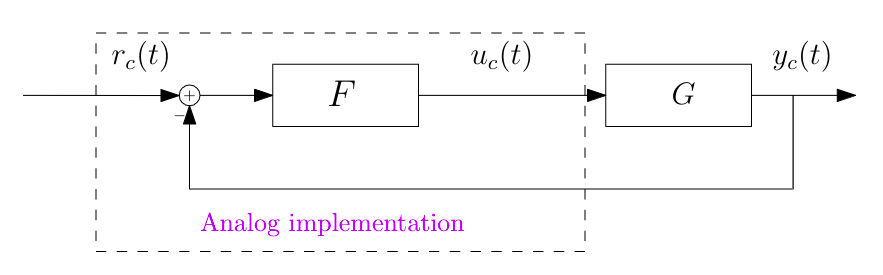
\includegraphics[width=12cm]{\imagesPath/digital_systems_and_discrete-time_clocks.png}
    \caption{Digital systems and discrete-time clocks. From \cite{}}
\end{figure}

\begin{figure}[!h]
    \centering
    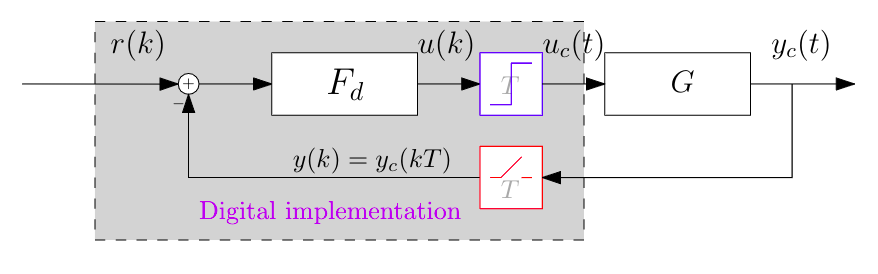
\includegraphics[width=12cm]{\imagesPath/digital_systems_and_discrete-time_clocks_da.png}
    \caption{Digital systems and discrete-time clocks. From \cite{}}
\end{figure}

\subsection{Sampling continuos-time output}
A/D: Sampling feedback signal $y(t)=y_c(kT)$

Nyquist sampling theorem:
If $y_c(t)$ is bandlimited to $\pm\omega_B = \pm2\pi f_b \Rightarrow$
it can be recovered exactly from $y_c(kT)$ when sampling frequency
\begin{equation*}
    f_s \equiv \frac{1}{T} > 2f_B
\end{equation*}

\newpage
\subsection{Generating continuous-time input}
Zero-order hold: continuos-time input is piecewise constant for $k=0,1,2,\ldots$
\begin{equation*}
    u_c(t) = u_c(kT), kT\leq t < (k+1)T
\end{equation*}

\begin{figure}[!h]
    \centering
    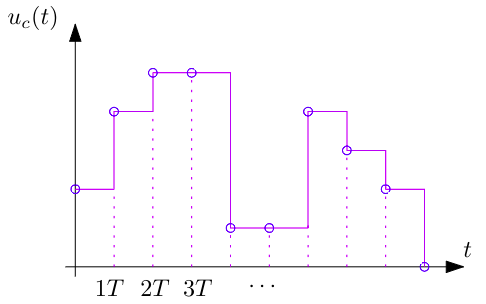
\includegraphics[width=12cm]{\imagesPath/zero-order_hold.png}
    \caption{zero-order hold. From \cite{}}
\end{figure}

\textbf{State evolution when using zero-order hold input} \newline
State $x_c(t)$ at time $(k+1)T$ is determined at time $kT$ as:
\begin{align*}
    x(k+1) &= Fx(k)+Gu(k) \\
    y(k) &= Hx(k)
\end{align*}
which are discrete-time states using matrices
\begin{align*}
    F &= e^{AT} \\
    G &= \int_{\tau=0}^{T} e^{AT} d\tau B = [\text{if } A^{-1} \text{ exists}] = A^{-1}(e^{AT}-I)B \\
    H &= C
\end{align*}

If eigenvalues of $A$: $Re(s) < 0 \Rightarrow$ stable

If eigenvalues of $F$: $|p|<1 \Rightarrow$ stable

\subsection{Discrete-time controllers}
PID controller 
\begin{equation*}
    u(k) = K_p e(k) + \underbrace{K_i T\sum_{n=0}^{k} e(n)}_{\simeq\int_{\tau=0}^te_c(\tau)d\tau} + \underbrace{K_d\frac{e(k)-e(k-1)}{T}}_{\frac{de_c(t)}{dt}}
\end{equation*}

\section{Final notes before exam}

Remember:
\begin{itemize}
    \item $G_0 = FG$ (useful when calculating the nyquist marginaly stable)
    \item poles of system in state space for is $\det{sI-A}$ 
    \item $Y(s) = G(s)U(s)$ logicaly
    \item $Y(s) = G_c(s)R(s)$ logicaly
    \item $G(s) = C(sI-A)^{-1}B$ 
\end{itemize}

Thing that were missing from the exam:
\begin{itemize}
    \item Forward- och cascade control (yes we have)
    \item Very little final value theorem
    \item What the diffrent PID parts does
    \item Roths algorithm
    \item Is the preformance spesifications met look at step response
    \item witch is the minimum phase
    \item general feedback control. is logical
    \item what is $F_r$ and $F_y$. use the formulas writen on exams. L9,p18
\end{itemize}

Other info:
\begin{itemize}
    \item (L3, P:) The system static gain is therefore $G(0)$ 
    \item (L3, P17) Stationary error $e_f$ approaches $0$ if $G(0)F(0) = \infty$. (E.g. when F(s) contains 1 s, i.e. integration.)
    \item (L5, P19) $G(s)=K_0\frac{\ldots}{\ldots}$
    \item (L6, P9) lead block lag block, formula is given in formula sheet
    \item (L6, P13) Among all systems G(s) with the same magnitude curve, the system with the least negative phase shift is a minimum phase system.
    \item (L8, P8) the close loop representation in state space form 
    \item (L8, P21) $G_c$ and $l_0$
    \item (L10, P6) Ideally S and T should be less then 1 but it is imposible since $|S(i\omega)|+|T(i\omega)|\geq 1$
    \item (L10, P9) Nyquist contour $G_o(i\omega) = F_y(i\omega)G(i\omega) = \frac{T(i\omega)}{S(i\omega)}$
    \item (L10, P11) Relative model error 
    \item (L10, P14) $|T(i\omega)| < \frac{1}{|\Delta G(i\omega)|}$ image
\end{itemize}
